% Surface EMG in Advanced Hand Prosthetics
% Castellini, van der Smagt
%
% Submitted to Biological Cybernetics, October/December, 2007
%
% Accepted for publication, March 2008
%

% notes to the reviewers, after producing the camera ready version:
%
% reviewer A
% ----------
%
% - the issue of sensorial feedback has never been in the scope of this
% work, so it would be impossible to deal with it now. nevertheless it
% is an important issue and you might be glad to know that we are
% thinking of starting a project in which bio-feedback is present. so far,
% we have added a reference to this issue in the ``discussion and
% conclusions'' section.
%
% - all other details have been taken into account by completely
% changing the abstract, intro and conclusions section. statements
% you judged too bold have been moderated, and one Figure which was,
% actually, not clear (and not necessary) has been removed.
%
% reviewer B
% ----------
%
% - abstract, intro and conclusions have been almost
% completely rewritten. the ``focus'' of the paper should now be
% clear: this is a preliminary study towards full control of an
% advanced hand prosthesis via EMG. the study was so far conducted on
% a healthy subject to test its feasibility, but of course it now
% needs to be tested upon amputees! we are hopefully going to start a project in
% which a hospital will be involved, and we hope we can, by then, show
% that it actually works.
%
% - the experimental results section, nr. 3, has been largely
% rewritten in order to avoid anecdotical writing; plus, we hope the
% hypotheses tested are clearer now.
%

% use option draft, final, or referee
\documentclass[twocolumn,referee]{svjour2}

\usepackage{times}
\usepackage{epsfig}
\usepackage{graphicx}
\usepackage{amsmath}
\usepackage[psamsfonts]{amssymb}
\usepackage{url}
\usepackage[pagebackref=true,breaklinks=true,letterpaper=true,colorlinks,bookmarks=false]{hyperref}

\def\RR{\mathbb{R}}
\def\NN{\mathbb{N}}
\def\xx{\mathbf{x}}
\def\yy{\mathbf{y}}
\def\ww{\mathbf{w}}

\begin{document}

\title{Surface EMG in Advanced Hand Prosthetics}

\author{Claudio~Castellini \and Patrick~van~der~Smagt}
\institute{
  Claudio~Castellini \at LIRA-Lab, University of Genova,
  viale F. Causa, 13, 16145 Genova, Italy,
  \email{claudio.castellini@unige.it}
  \and
  Patrick~van~der~Smagt \at Institute of Robotics and Mechatronics,
  German Aerospace Center/DLR, Oberpfaffenhofen, Germany,
   \email{smagt@dlr.de}
}

\maketitle

\begin{abstract}
  abstract
\cite{v-edbed-82}

\end{abstract}

\keywords{
Learning and Adaptive Systems; Rehabilitation Robotics; Physical
Human-Robot Interaction
}

\section{Introduction}
\label{sec:introduction}
Active prosthetic hands, driven by a motor to open and close the
``claw,'' have been around for many years.  Recently, however,
advances in mechatronics have improved such hands and currently
various prosthetic hands with 3 or more active degrees of freedom are
being put on the market.  Such hand developments are a result of
various robotic hands which are highly humanoid, light and gifted with
a number of degrees of freedom. Attempts in this sense include, e.g.,
the DLR prosthetic hand (\cite{Hua2006}---see Figure
\ref{fig:DLRHandII}), the CyberHand project \cite{cyberhand}, and the
i-LIMB hand by Touch Bionics \cite{ilimb}.

\begin{figure}
  \begin{tabular}{cc}
    \includegraphics[height=0.12\textheight]{figs/DLRHand-Ball-comp.jpg} &
    \includegraphics[height=0.12\textheight]{figs/DLR-Prothese.jpg}
  \end{tabular}
  \caption{(left) The DLR Hand II. (right) The DLR prosthetic hand.}
  \label{fig:DLRHandII}
\end{figure}

Still, a general sense of frustration impends, as far as
\emph{control} of the prosthesis is concerned. As a matter of fact,
given the current state of the art, it is basically impossible for the
patient to precisely command the prosthesis what to do; whereas,
operating a hand requires a fine control down to the level of the
single fingers. First of all, presented with a certain task such as
turning a door handle or grabbing a car key, the patient must be able
to enforce the correct grasping type; this involves the activation of
some joints only, and in particular positions. Secondly, the amount of
force involved in the grasp must be controlled, so that it is possible
to grab, e.g., both a hammer without letting it slip and an egg
without breaking it.

To this end, two types of interfaces between the patient and the
prosthesis have been developed or are being studied: \emph{invasive}
and \emph{non-invasive}. The former gather control signals directly
from the user's nervous system, either via brain implants or surgical
use of electrodes. Quite obviously, invasive interfaces are supposed
to deliver a high signal quality, since the signals can be gathered
exactly in the right spots; but they involve surgery and all related
sterility (and psychological) issues. On the other hand, non-invasive
interfaces are easier to handle, manufacture and implant, but require
a much better signal conditioning, since they usually work with
surface (skin) signals or vision and gaze tracking.

In the context of non-invasive interfaces for controlling mechanical
hands, a concrete possibility arises from \emph{forearm surface
electromyography} (EMG), a technique by which muscle
activation potentials are gathered by electrodes placed on the
patient's forearm skin; these potentials can be used to track which
muscles the patient is willing to activate, and with what force.
Surface EMG is therefore, in principle, a cheap and easy way of
detecting what the patient wants the prosthesis to do.

Still, the EMG signal suffers from a number of problems, among which
the unprecise placement of the electrodes, signal drifting and change
due to sweat formation and muscular fatigue and cross-talking among
deep and superficial muscles. It seems, though, that good results can
be obtained via \emph{machine learning} techniques, as shown in, e.g.,
\cite{smagt}. In machine learning, one tries to approximate an unknown
function given its values in a number of samples; the application to
the current problem is exactly that of building a map relating EMG
activation potentials and muscle force, and therefore hand finger
movements.

Such a system must be highly adaptive, accurate and fast---possibly,
able to run in real time, as the patient is wearing the prosthesis.
Another very desirable characteristic is that the system should learn
automatically as the patient moves, being able to understand when new
portions of the input space are being explored, i.e., what new
movements are required of the prosthesis. But so far machine learning
applied to surface EMG has only been able to classify hand postures.
For example, the surface EMG signal can be used to detect whether the
patient is attempting a cylindric grasp or a two-finger grip
\cite{ekvall}; but no indication about the amount of force involved in
the grasping act is detected.

In this paper we show a rather detailed analysis of what machine
learning can do when applied to such a problem. Over several days, we have
gathered forearm surface EMG data while an able-bodied human subject
was gripping in four distinct ways a force sensor; we have then
trained three different machine learning systems to guess, from the
EMG signal,
\begin{enumerate}

  \item what kind of grasp the subject was doing, e.g., thumb and
    index finger, thumb and middle finger, thumb and ring finger or
    thumb and all other fingers; and

  \item how much force the subject was exerting, in order to
    understand whether the grasp was, e.g., a power grasp or rather a
    precision grip. Surprisingly, as far as we know, nobody has ever
    attempted so far to solve this problem, although it is well-known
    that the EMG is related to the force a muscle is exerting.

\end{enumerate}

The three approaches we have experimented with are:
(a) a simple feed-forward neural network with one hidden layer,
(b) a Support Vector Machine with radial basis function kernel
\cite{BGV92}, and (c) Locally Weighted Projection Regression
\cite{lwpr}. Our analysis consists of a preliminary phase in which
several models have been built in a batch fashion, in order to
understand how to deal with the non-stationarity of EMG. The most
interesting challenge has been how to filter out unwanted data, at the
same time keeping a high overall accuracy, both in classification and
regression. Later on, based upon the results obtained in the
preliminary phase, we have developed a simple but effective procedure
for selecting a subset of the samples on-the-fly, called \emph{Online
Uniformisation} (OU).

OU is based upon the simple idea of keeping a minimum inter-sample
Euclidean distance, in order to uniformly sample the input space. The
selected samples are then used to periodically re-train the system,
and check that it has adapted to the new data. The training sets thus
obtained are remarkably small and thus usable on-line, and they offer
an excellent trade-off between size and accuracy. In particular, as a
certain parameter is increased, the size of the uniform training sets
decreases polynomially, while the error rate increases only
linearly; therefore one can obtain much smaller training sets (which
means faster or more adaptive machines) by accepting an error rate
which is only linearly worse.

This behaviour appears in both problems highlighted above (the former
involving classification, the latter regression), and for all the
approaches tested. Our numerical results indicate that, in such a
scenario, the type of grasp can be reconstructed with an average
accuracy of $89.67\% \pm 1.53\%$, and the applied force can be
predicted with an average percentage error of $7.89\% \pm 0.09\%$,
meaning $4.5$N over a range of about $57$N.

The paper is structured as follows: after a brief review of relevant
literature, we describe in detail the experiment and the methods used
to tackle it (Section \ref{sec:m&ms}); then we show and comment on the
experimental results, both the preliminary phase and the online
experiments (Section \ref{sec:exp}); lastly, discussion and
conclusions are presented.


\subsection{Related Work}
\label{subsec:relatedwork}
related work.

do we really want to have this section? if so:

\textbf{[[1.Patrick will you help here. do we want to have something
about the forthcoming DLR hand, and how one can in principle control
it using a force signal such as the one we can predict from the EMG?]]}

\textbf{[[2.Patrick again: what approaches have been used in
literature to interface EMG and prosthetic hands, NOT LIMITED to
machine learning?]]}



\section{Materials and Methods}
\label{sec:m&ms}

In this Section we describe the experiment we have conducted and the
methods we have employed to gather the data, filter and analyse them.

\subsection{Experimental Setup and Design}
\label{subsec:setup}
The aim of the experiment was to gather forearm surface EMG data in
real-time, and to relate it to $(a)$ the type of grasp applied by the
subject, $(b)$ the force applied by the subject while grasping.

\subsubsection{General setup description}

The experiment consisted of freely, repeatedly pressing a SpaceControl
OFTS force/torque sensor \cite{...} along the large face. Four
different ways of pressing were allowed: opposing the thumb and index,
the thumb and middle, the thumb and ring or the thumb and all other
fingers, at different speeds and with varying force. Four force-sensor
resistors were applied on the subject's hand fingertips (thumb, index,
middle and ring), in order to be able to detect which grasp type was
used at each instant of time. At the same time, $10$ forearm surface
EMG electrodes were applied to the subject's forearm, in order to
gather information about the muscle activation. Figure \ref{fig:setup}
shows some parts of the setup.

\begin{figure*}[!ht] \centering
  \begin{tabular}{ccc}
    \includegraphics[height=0.16\textheight]{figs/OFTS} &
    \includegraphics[height=0.16\textheight]{figs/ottobock} &
    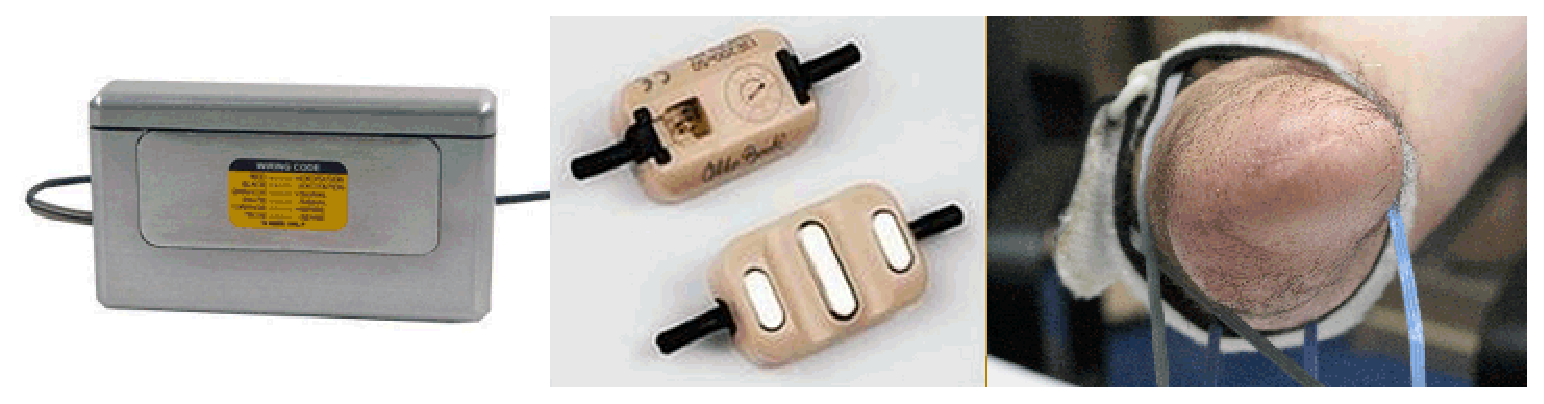
\includegraphics[height=0.16\textheight]{figs/setup} \\
    $(a)$ & $(b)$ & $(c)$ \\
  \end{tabular}
  \caption{The experimental setup. $(a)$ The SpaceControl OFTS
    force/torque sensor, large face up. $(b)$ An Otto Bock 13E200=50
    surface EMG electrode, with the amplification gauge (upper part of
    the Figure) and the three metallic contacts (lower part). $(c)$
    The arm of the subject with the EMG electrodes fitted and held in
    place by elastic bands. Electrodes cables are wired in a box and
    then directed to a National Instruments PCI-6023E analogic/digital
    conversion card (not shown).}
  \label{fig:setup}
\end{figure*}

Numerical data from the EMG and fingertip sensors were gathered at a
sampling rate of $256$Hz using a National Instruments DAQ PCI-6023E
analogic/digital conversion card \cite{...}, mounted on a fast PC
equipped with Windows XP. Data coming from the OFTS sensors was
gathered via the serial port. We ensured that the sampling rate was
high enough and that the card and serial port would respond properly
when requested for data. The data were subsequently synchronised and
saved onto files.

\subsubsection{EMG signal and electrode placement}

The $10$ EMG electrodes were applied to the subject's right forearm,
held in place by elastic bands. The electrodes were
double-differential Otto Bock 13E200=50 models \cite{...}, each one
gifted with an amplification gauge ranging from $2000$ to $100000$
times. Initial qualitative experiments revealed that a safe setting
for the amplification gauge was in the middle of the range,
corresponding to about $14000$ times. This is in agreement with the
EMG signal amplitude predicted in the related literature (see, e.g.,
\cite{deluca}), that is about $100 \mu V$ on average: the voltages our
DAQ card read ranged from slightly more than $0V$ to $3V$.

Six of the electrodes were placed in pairs along the lower face
of the forearm, whereas four of them were applied in pairs on the
upper face. The initial positioning of the electrodes was chosen
following an anatomical guideline \cite{...} in order for them to lie
approximately on top of the muscles which elicit finger movements. As
well, we were inspired by the placement description in \cite{smagt},
which proved to be optimal for Support Vector Machine classification
of hand postures.

As far as the EMG signal is concerned, it must be remarked that it is
subject to remarkable changes depending on, at least, four orders of
factors:

\begin{enumerate}

  \item \emph{the subject.} All forearms are different from one
    another in shape, size and power.

  \item \emph{arm posture.} Besides finger movements and grasping, the
    forearm muscles are also involved in the motion of the arm. The
    EMG signal is therefore likely to change if the forearm is moved
    during signal acquisition, for example when switching from
    pronation to supination.

  \item \emph{electrode placement.} The intensity and quality of the
    EMG signal depends upon a correct placement of the electrode over
    a muscle. In principle, each electrode should be placed over a
    single muscle, precisely on top of the muscle belly, halfway the
    length of the muscle, and always exactly in the same place.

  \item \emph{muscle fatigue.} As the muscles are used more and more,
    continually, fatigue changes the RMS of the EMG signal, calling
    for continual adaptation, at least over a reasonable set of
    different fatigue conditions.

\end{enumerate}

As far as the first problem is concerned, since in a real setting one
person only is expected to train and wear the prosthesis, we have not
investigated multi-subject feasibility of the approach, concentrating
on one subject only, male, aged $35$ and fully able-bodied. Of course,
further investigation is required to check whether the approach can be
transferred to real amputees, by exploiting the residual potential
muscular activation left in their forearm stump. Moreover, independent
multi-subject analysis will have to be carried on, in order to check
that the described approach works with the same accuracy results for
any human being.

In order to overcome the second problem, we instructed the subject to
keep the arm still and relaxed on a table in a confortable position,
with the palm orthogonal to the plane of the table.

Lastly, as far as muscle fatigue and electrode displacement are
concerned: in general, electrodes \emph{cannot} be expected to exactly
lie in the very same position every time the prosthesis is used;
moreover, in a preliminary round of experiments, muscle fatigue was
clearly perceived by the subject during the experiment. In this
framework, the only possibility to overcome these problems is to
explicitly take them into account, gathering enough data to be able to
train the machine under different conditions of electrode displacement
and muscular fatigue.

We then organised the experiment as follows: the subject was
instructed to continually grasp the sensor over a period of time of
three to four minutes; then he was allowed to rest for about two
minutes. This was called a \emph{session}. It was expected that muscle
fatigue would appear already during one session.

Three sessions were gathered without taking the elastic bands off the
subject's forearm, in order \emph{not} to have electrode displacement
within a set of three sessions, that we called a \emph{group}. After
each group, the electrodes and bands were removed and the subject was
allowed for a much longer period of rest, ranging from half an hour to
one hour. During resting in-between groups, the subject could get back
to his normal muscular activity.

Five groups were then gathered during one day; and this procedure was
entirely repeated during another day. This procedure would allow us to
examine a relevant amount of data, gathered along a relatively long
period of time and inder different conditions of muscle fatigue
(within one session) and electrode displacement (between groups).

As an example, Figure \ref{fig:drift} shows the output of electrode
$8$ during three different sessions: $1$ and $2$, belonging to the
same group, and $7$ (moving average over about $10$ seconds). One can
notice strong low-frequency components, essentially drifts due to
muscle fatigue.

\begin{figure*}[!ht] \centering
  \begin{tabular}{ccc}
    \includegraphics[width=0.32\textwidth]{figs/el8_movingAvg_s1} &
    \includegraphics[width=0.32\textwidth]{figs/el8_movingAvg_s2} &
    \includegraphics[width=0.32\textwidth]{figs/el8_movingAvg_s7} \\
    session $1$ & session $2$ & session $7$ \\
  \end{tabular}
  \caption{Typical behaviour of an electrode signal over different
  sessions (moving average over about $10$ seconds. Drifting can be
  clearly seen in the signal, due to muscle fatigue.}
  \label{fig:drift}
\end{figure*}

\subsubsection{Force applied during the grasp}

The OFTS force/torque sensor would output a (negative) numerical value
ranging from $0$ to about $5000$, expressed in fiftieths of a
Newton. After normalisation, the range would be between $0N$ and
$50N$.

\subsubsection{Type of grasp}

The values output by the $4$ force resistor sensors applied onto the
subject's fingertips were monitored in order to understand which kind
of grasp the subject was applying to the sensor. A threshold was
experimentally decided, above which the finger would be in contact
with the sensor. Using this technique, for each instant in time one of
five possible categories was established: $0$, no action; $1$,
grasp by opposing the thumb and index finger; $2$, opposing thumb and
middle; $3$ thumb and ring; and lastly, $4$ grasp by opposing the
thumb and all other fingers.

It must be remarked here that the EMG signal would be altered
immediately at the onset of finger movement, which our setup was
unable to detect. This would result in potential noise in the
categorisation of category $0$.

Figure \ref{fig:targets} shows typical values of the OFTS sensor and
the related categories. One can clearly see that the applied force is
in general higher when grasp type $4$, all fingers involved, is used,
as expected.

\begin{figure*}[!ht] \centering
  \begin{tabular}{cc}
    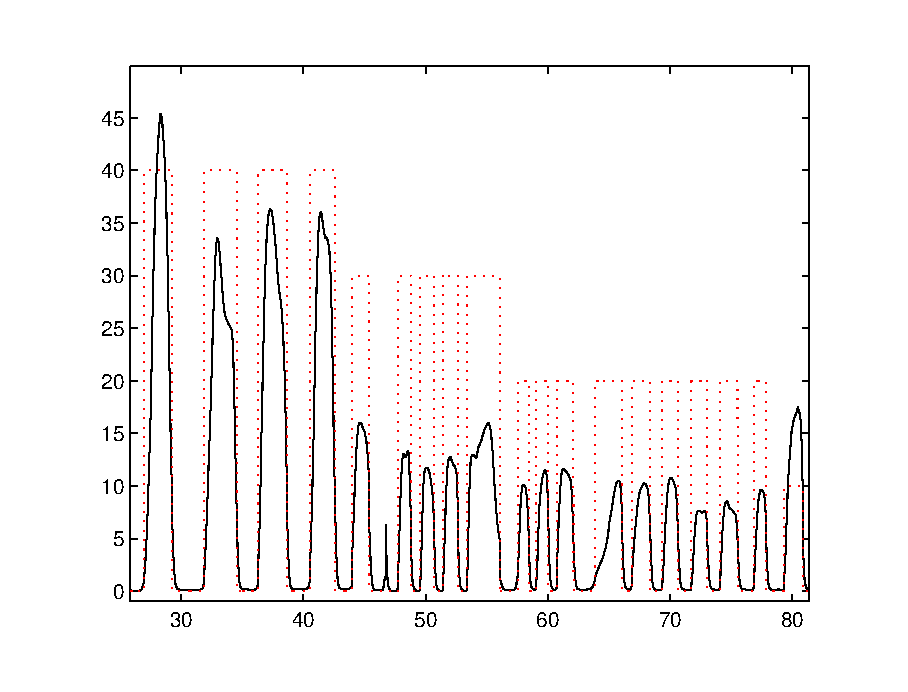
\includegraphics[width=0.45\textwidth]{figs/targets_zoom1} &
    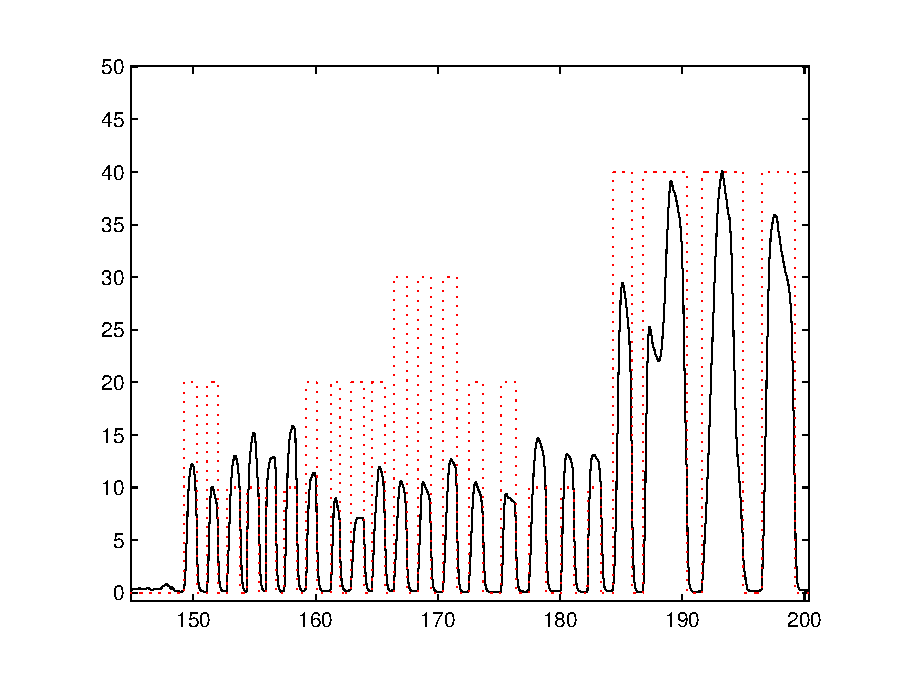
\includegraphics[width=0.45\textwidth]{figs/targets_zoom2} \\
  \end{tabular}
  \caption{Typical values output by the OFTS sensor (black line), and the
    categories evaluated from the fingertip sensors values (red
    line). The Figures are zooms of the same session.}
  \label{fig:targets}
\end{figure*}


\subsection{Learning Methods}
\label{subsec:analysis}
The gathered data was analysed both for classification and
regression. \emph{Classification} is the process by which one wants to
assign a label to each sample in the input space, whereas in
\emph{regression} the target is a real-valued function of the values
of the input samples. Throughout this Section, we will assume that a
set of $l$ points in the input space is available, for which the
target (label or force value) is known; this set will be denoted by
$\{\xx_i,y_i\}_{i=1}^l$ and called \emph{training set}. As well, for
each experiment, a separate set of points, for which the targets are
not known, is assumed to be available, and this will be called the
\emph{testing set}. In general, the performance of a machine is tested
by training it on a training set and then testing it on a testing set,
possibly employing standard measures of the generalisation error, such
as cross-validation.

Taking into account the considerations of the previous Section, we set
the input space to be $\RR^{10}$, that is, one coordinate for each EMG
electrode; therefore, $\xx_i \in \RR^{10}, i=1,\ldots,l$. In the case
of classification, each category representing a grasping type would be
represented as an integer value, that is, $y_i \in \{0,\ldots,4\}
\subset \NN, i=1,\ldots,l$. In the case of regression, the force value
would be directly encoded as a real number, that is, $y_i \in \RR,
i=1,\ldots,l$. Before any analysis, all samples were normalised, as is
customary, by subtracting the mean values and dividing by the standard
deviation, for each input space dimension. No filtering whatsoever was
applied to the input signals, in order to have a more realistic,
delay-free result.

\subsubsection{Neural Networks}

Artificial Neural Networks (NNs or ANNs for short; see, e.g.,
\cite{bishop} for a comprehensive introduction) are probably the most
popular machine learning algorithm nowadays available for both
classification and regression. An ANN is a directed graph in which,
for every node, the weighted sum of the input values is evaluated;
this sum is then used as the argument of an \emph{activation function}
to determine the output of the node. The nodes fed the input values to
the network are called \emph{input layer}, and the nodes whose output
is taken as the output of the network are called \emph{output
layer}. Besides this, in general, an ANN can further have an arbitrary
number of nodes organised in \emph{hidden layers}, gifted with an
arbitrary edge topology.

An ANN is initialised with random weights; then, for every sample in
the training set, the network output is evaluated and its error with
respect to the target is considered. In order to reduce the error
then, a minimisation algorithm is then employed to change the weights
of the network, until the desired precision is reached. If the
generalisation error has been kept small, the network will then be
able to \emph{predict} the targets of the testing samples with a
reasonable accuracy.

For our experiment we strived to keep the ANN as simple as possible.
We then chose a basic feed-forward NN with $10$ units for the input
layer; one hidden layer with $10$ units with sigmoidal arcotangent
activation function; $5$ units in the output layer for classification,
each unit representing one category, and one unit in the output layer
for regression, the unit representing the target force value. The
network was trained via the \textbf{BOH} algorithm and learning
function \textbf{BOHBOH}; the mean-square error (MSE) was used as a
measure of performance. The training phase was stopped arbitrarily
after $30$ epochs. For each experiment, we repeated the training phase
$10$ times, in order to overcome the well-known problem of local
minima, and then gathered the best model found. No measure of
generalisation error was taken into account.

The network was implemented in Matlab, Windows version $7.1.0.246$
(R14) Service Pack 3, running on a bi-processor $1.8$GHz machine with
1GB on-board memory; we used the Matlab Neural Network Toolbox,
version $5.0.1$ (R2006b).

\subsubsection{Support Vector Machines}

Support Vector Machines (SVMs; see, e.g.,
\cite{BGV92,Burges98,Cristianini00}) are a machine learning method
able to determine the best candidate function for a classification or
regression problem, drawn from a functional space induced by the
choice of a binary function between points in the sample space,
$K(\xx_1,\xx_2)$, with $\xx_1, \xx_2 \in \RR^{10}$ in this case. $K$
is called \emph{kernel}. In the most general setting, the function
found is

\begin{equation} \label{eqn:sol}
  f(\xx) = \sum_{i=1}^l \alpha_i y_i K(\xx,\xx_i) + b
\end{equation}

\noindent where $b \in \RR$, whereas the $\alpha_i \in \RR$s are
Lagrangian coefficients obtained by solving a minimisation problem
whose cost functional is guaranteed to be convex. Because of this,
SVMs do not suffer from the problem of local minima; but their
training time is cubic in the number of samples in the training set,
as opposed to ANNs, for which it is \textbf{BOHBOH}.

In order to overcome this problem, which would have made our
experiment unfeasible, we have decided to use a \emph{uniformisation}
strategy on the training sets, before training the machines. The idea
is that, in a real-life set-up such as ours, there can be many input
samples located in the very same region of the input space, with very
similar target values. One obvious case is that of label $0$,
indicating no ongoing grasping: it is intuitively expected that a
large number of samples will be taken in that region of the input
space, since the subject will be in the $0$ condition for a longer
time than all other labels.

Since all functions involved in the experiment are due to human
motion, we can assume that they are continuous and, probably,
derivable up to any arbitrary order. Therefore it makes no sense for
an approach such as SVMs to sample the input space in a non-uniform
way such as that described above. The uniformisation procedure
consists of removing, from a training set, those samples which are too
close to each other, according to a suitable notion of inter-sample
distance.

In order to take into account the different variances of the EMG
electrode values, we have decided to adopt Mahalanobis's distance as
the inter-sample distance \cite{...}. Let $\xx_1, \xx_2 \in \RR^{10}$;
then the Mahalanobis distance between $\xx_1$ and $\xx_2$ is defined
as follows:

$$ MD(\xx_1,\xx_2) = \sqrt{(\xx_1-\xx_2)^T \Sigma^{-1} (\xx_1-\xx_2)} $$

\noindent where $\Sigma$ is the $10$x$10$ covariance matrix, evaluated
on the training set. $MD(\xx_1,\xx_2)$ is a distance in which each
summand is weighted inversely with respect to the variance of the
samples along that dimension of the input space: it is therefore a
measure of distance independent of the variance of the single
electrodes. Notice that if $\Sigma$ is replaced by the identity
matrix, $MD(\xx_1,\xx_2)$ is reduced to the usual notion of Euclidean
distance.

Since checking the inter-sample distance obviously takes a quadratic
time with respect to the number of samples, which was unfeasible, we
adopted an approximated method which was able to remove most, but not
all, samples with an insufficient Mahalanobis distance from any other
sample. After a few initial experiments we set the threshold distance
at $1$. All our experiments with SVMs were then performed on
uniformised training sets, using $5$-fold cross-validation and grid
search to find the optimal values of the standard Gaussian kernel
hyperparameters, $C$ and $\sigma$.

On the other hand, notice that no \emph{testing} set was uniformised,
since it would probably be unfeasible to apply the same procedure in
an on-line setting. Notice, further, that applying uniformisation
resulted in training sets which were considerably smaller than the
original ones, up to about $100$ times smaller.

Lastly, we employed a well-known freely available SVM package,
\emph{libsvm} v2.83 \cite{...}, in the Matlab wrapped flavour.

\subsubsection{Locally Weighted Projection Regression}

\textbf{LWPR - prendi qualcosa dalla rete. spiega gs e cv.}



\section{Experimental Evaluation}
\label{sec:exp}

In this Section we describe the experimental analysis. In particular,
we first describe some preliminary results obtained in batch fashion,
which have led to the development of Online Uniformisation (OU). We
then show a detailed comparative analysis of the three approaches
selected, first on the classification problem, and then on the
regression problem, in which OU is used.

\subsection{Batch Experiments}
\label{subsec:strategy}
%When dealing with a signal such as the EMG, subject to wide variations
%due to external effects, and thinking of the final application, that
%is a prosthesis eventually sold to and worn by a patient, we had to
%devise a strategy to correctly build a training set for our
%machines. In particular, a way of gathering samples from relevant
%zones of the input space must be thought of. The term \emph{relevant}
%here is used informally to mean ``such that further use of the system
%will involve samples drawn from the same zone''.
%
%In particular, see Section \ref{subsec:setup}, the final user will be
%using the prosthesis under various conditions of muscle fatigue,
%electrode displacement and arm motion. The organisation of data
%gathering into sessions, groups and days helped us collect enough
%data, it was expected, to overcome the first two problems, while we
%explicitly neglected the third, to be investigated in further
%research. It remains to understand how to use the data actually
%gathered to build a model which will generalise well, that is, trained
%upon a relevant zone of the input space.

\subsubsection{Uniformisation}

First of all we chose one of the selected approaches (NNs, SVMs or
LWPR) and one problem (classification or regression) for initial
experimentation. We decided to use SVMs for classification. We then
decided to test whether data obtained during one session could be used
to build a model able to generalise over other sessions during the
same day. At the same time, we wanted to check whether the
uniformisation procedure (see Section \ref{subsec:analysis}) would be
effective in reducing the training set, at the same time without
losing relevant information.

Therefore, we trained a SVM over each single session, both for the
first and second day, and both with full and uniformised training
sets. The session were numbered chronologically during the day,
sessions $1,2,3$ forming group $1$, sessions $4,5,6$ forming group
$2$, and so on. With a slight abuse of language, we will call the
model obtained by training a machine on session $i$, \emph{model
$i$}. Moreover, in the remainder of this Subsection, if the training
set of a model was uniformised, we will call the model \emph{uniform}.

We then tested each model on all sessions of the same day, obtaining
an \emph{accuracy matrix} $A$ in which $A_{ij}$ would be a percentage
denoting the correctly guessed labels when testing model $i$ (standard
or uniform) on session $j$. Notice once again that, in the case of
uniform models, the test is carried out on the \emph{full}
session. This is what we would call a \emph{cross-session analysis}.
The result is visible in Figure \ref{fig:cross_initial}.

\begin{figure} \centering
  \begin{tabular}{cc}
    \includegraphics[width=0.22\textwidth]{figs/fig_resCross1_full} &
    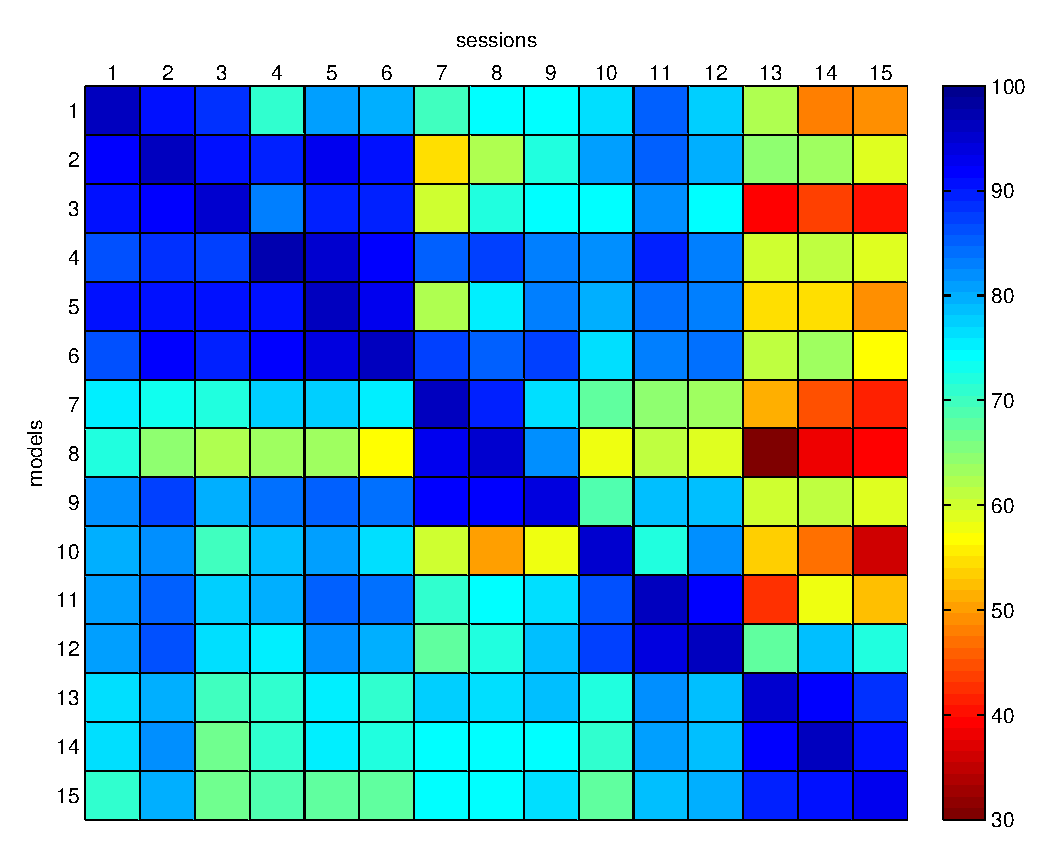
\includegraphics[width=0.22\textwidth]{figs/fig_resCross1} \\
    (a) diag: $98.73\% \pm 0.39\%$  & (b) diag: $95.52\% \pm 1.21\%$ \\
        rest: $73.23\% \pm 14.29\%$ & rest: $74.53\% \pm 13.70\%$ \\
    \includegraphics[width=0.22\textwidth]{figs/fig_resCross2_full} &
    \includegraphics[width=0.22\textwidth]{figs/fig_resCross2} \\
    (c) diag: $99.05\% \pm 0.37\%$ & (d) diag: $95.37\% \pm 2.85\%$ \\
        rest: $73.23\% \pm 14.47\%$ & rest: $74.38\% \pm 12.27\%$ \\
  \end{tabular}
  \caption{Cross-session analysis and evaluation of the uniformisation
    procedure. $(a)$ and $(b)$, accuracy matrices for day $1$: $(a)$
    full models, $(b)$ uniform models. $(c)$ and $(d)$, same for day $2$.}
  \label{fig:cross_initial}
\end{figure}

Consider first panes $(a)$ and $(b)$ of the Figure, pane $(a)$
being the accuracy matrix for full models, day $1$, and pane $(b)$
being the accuracy matrix for the same day, but using uniform
models. It is apparent from the shades that the full models attain
a better accuracy when tested on their own training data, that is,
on the diagonal of the matrix, than the uniform models.  This is
intuitively sensible since, in the case of full models, we are
testing on the same data used for training, whereas in the case of
uniform models, the training data are a strict subset of the
testing data, and a quite smaller subset indeed. But as well, if
we consider the remaining elements of the matrices, it is clear
that the uniform models attain a better accuracy \emph{overall},
if compared to the full models. The same analysis for day $2$
(same Figure, $(c)$ and $(d)$) yields analogous results.

From this we conclude that the uniformisation procedure is effective
in reducing the training set size, without actually degrading the
performance. This is apparent from the fact that uniform models are
more accurate on testing sets which are disjoint from the training
sets. In fact, one should always ensure that this is the case, aiming
for a better generalisation error. We can say that uniform models
generalise better, at least in this case.

Therefore, from now on, all models we will be using, in the case of
SVMs and LWPR, will be the uniform ones.

\subsubsection{Classification accuracy}

Consider Figure \ref{fig:cross_initial} again, panes $(b)$ and
$(d)$. The accuracy attained on non-diagonal elements is about
$74\%$, which is rather bad. One cannot expect to correctly drive
a prosthesis if one sample in four is misclassified. At the same
time, however, a strong ``good group accuracy'' is obviously
present: in each matrix, good accuracy values are obtained on
$3\times3$ submatrices located on the diagonals, corresponding to
cross-session accuracy for sessions \emph{belonging to the same
group}, that is, where the elastic bands were not removed and no
electrode displacement was present.

More in detail, as far as the first day is concerned (same Figure,
pane $(b)$), one can see that the first six models (trained on the
first two groups) obtain a quite good accuracy on the first six
sessions (first two groups) whereas their accuracy rapidly degrades as
more sessions are tested for. This is probably due to the first two
groups having been gathered in similar conditions, very similar
electrode positions and/or similar movements performed by the
subject. On the other hand, sessions in the last group (columns $13$,
$14$ and $15$ of the matrix) are particularly hard, except when tested
by models obtained from the last group itself---here the effect is
motivated by the opposite reason: during those sessions, the subject
must have explored more relevant parts of the input space. This is
corroborated by the fact that models $13,14,15$ perform rather well on
\emph{all} sessions, if compared to other models (check rows
$13,14,15$ of the matrix). In other words, sessions $13,14,15$ contain
more relevant information than the others.

Analogous considerations can be made by inspecting the accuracy matrix
of the second day, pane $(d)$ of the Figure.

From this we can confirm that \emph{electrode displacement plays a
determinant role} in the classification accuracy. Notice that
muscle fatigue seems not to enter the picture, but this is
reasonable since its effetcs are visible already within one single
session and the machine correctly takes it into account during the
training phase. Notice once again that the uniformisation
procedure does not hinder the generalisation power of the system.

%It is intuitively expected that the poor cross-session generalisation
%performance is due to the problem of electrode displacement. This is
%experimentally confirmed by the strong degradation in classification
%accuracy among different groups. In other words, the SVM does not
%generalise well when trained on a session belonging to group and
%tested on a session belonging to a different group.
%
%Poor generalisation is often due to the samples in the training and
%testing sets being drawn from two different probability distributions
%or from two essentially different zones of the input space. We claim
%that this is the case. \textbf{[[PATRICK: I know this sounds quite
%wobbly. can you say it in a more precise way, possibly with
%citations?]]}

%In particular, we hypothesise that the electrode displacement present
%between groups (but not within a group) causes the samples in a group
%to be ``shifted'' in the input space, so that testing on a different
%group results in poor generalisation performance. To substantiate this
%claim, we have verified that the cross-session accuracy is highly
%correlated to the \emph{average minimum inter-sample distance} between
%sessions. More in detail, let $S_i$ denote the training set for
%session $i$; we have built a distance cross-session matrix $D$ in
%which
%
%$$ D_{ij} = \frac{1}{|S_j|} \sum_{s_j \in S_j}{\min_{s_i \in S_i}{ ||s_j-s_i||^2 } } $$
%
%Essentially, $D_{ij}$ denotes how far away in the input space the
%samples in $S_j$ are from the samples in $S_i$. Note that $D$ is in
%general not symmetric, since we consider the \emph{average} of the
%\emph{minimum} distance of each sample in $S_j$ from those in $S_i$.
%
%The cross-correlation coefficient evaluated between the values of $D$
%and the accuracy values of the cross-session accuracy matrix is
%$-0.61$ \emph{both} for the first and the second day, indicating a
%strong negative correlation. Further experiments have revealed that
%this happens for Neural Networks too (cross-correlation $-0.40$ for
%day $1$ and $-0.51$ for day $2$); and also, that $D$ is strongly
%\emph{positively} correlated to the MSE in regression, for all the
%studied approaches: $0.62/0.78$ (day $1$/day $2$) for SVMs,
%$0.64/0.72$ for NNs and $0.77/0.81$ for LWPR.
%
%In other words, the larger the distance of $S_i$ and $S_j$, the worse
%the performance of model $i$ tested on session $j$, both in
%classification and in regression. This tells us that $(a)$ samples of
%the same group are closer to each other than sample from different
%groups, therefore electrode displacement causes displacement in the
%input space too; and $(b)$ that this causes bad inter-group
%performance. ``Samples far away from the training set will be
%predicted badly.''
%
%In order to further sustain this claim we have checked, for each day,
%that models obtained by adjoining $4$ of the $5$ groups would perform
%well on the group excluded when training; this would indeed indicate
%that more data is needed to train the machine, and that the required
%data must somehow be found in some of (but not necessarily all) the
%gathered groups. We will call these models \emph{multi-group
%models}. The results are visible in Figure \ref{fig:bigmodels}.
%
%\begin{figure*}[!ht] \centering
%  \begin{tabular}{cc}
%    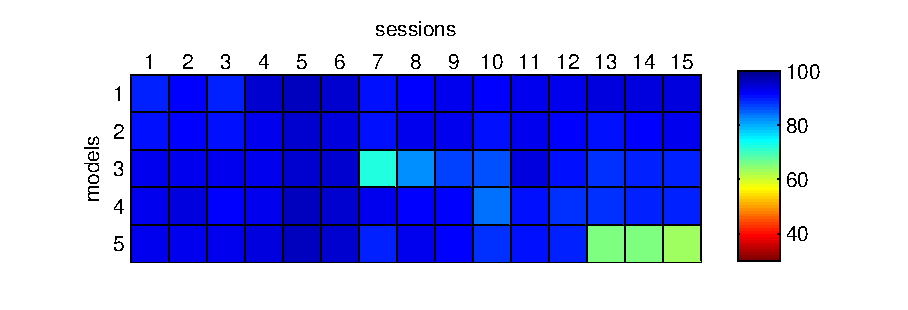
\includegraphics[width=0.45\textwidth]{figs/fig_resCross_day1_big} & \includegraphics[width=0.45\textwidth]{figs/fig_resCross_day2_big} \\
%    $(a)$ & $(b)$ \\
%  \end{tabular}
%  \caption{Cross-session analysis of multi-group models, obtained by adjoining $4$
%    of the $5$ groups of each day. Each row denotes the model trained
%    excluding group $1,\ldots,5$ from the model itself. $(a)$ day $1$, $(b)$ day $2$.}
%  \label{fig:bigmodels}
%\end{figure*}
%
%Consider the rows of the matrices in the Figure: as one can see, the
%accuracy is uniformly very high, even when the models are tested on
%unseen testing data; for instance, model $1$ of day $1$ has an
%accuracy of $92.82\% \pm 1.96\%$, and model $4$ of day $2$ has an
%accuracy of $92.64\% \pm 3.73\%$. Moreover, notice that, e.g., model
%$5$ of day $1$ performs badly on group $5$ of day $1$, as one can
%expect, since model $5$ has not been trained on that very group, which
%was already determined to be very hard (compare Figure
%\ref{fig:cross_initial}, pane $(b)$, last three columns).
%
%On the other hand, this analysis proves that if we train upon the
%``right'' data, the accuracy becomes acceptable. Model $1$ of day $1$,
%for instance, performs uniformly very well. From this we first
%conclude that the uniformisation procedure is not eliminating any
%useful information from the training sets; and, secondly, that if the
%right training data can be found, there are good chances of building a
%good model.

\subsubsection{Best models}

Lastly, we have considered how to collect \emph{only} relevant
information from the gathered data, that is, how to sensibly reduce
the training set. To do this, we have collected the two best models
for each day and joined them together. For instance, consider Figure
\ref{fig:cross_initial} again, pane $(b)$. It is apparent that model
$4$ performs well on sessions $1$ to $12$, whereas model $13$ does
well on sessions $13$ to $15$. We then decided to use these two models
to form a ``best'' training set which would give good results on the
whole day $1$. Analogous considerations led us to use also models $4$
and $8$ of day $2$. The obtained model will be called \emph{best}
model.

This procedure was repeated for each problem tackled
(classification, regression) and approach tested (NN, SVM, and
LWPR). The results are presented below.


\subsection{Online Experiments}
\label{subsec:online}
The considerations of the previous Subsection lead to the reasonable
hypothesis that inter-sample distance is the key. Keeping training
sets uniform will result in smaller sets which still contain all
information required for training. Moreover, bad generalisation is
correlated to inter-set distance; therefore uniformisation can be as
well used to retain samples which are far away from the current
training set. We have then implemented an online version of the
uniformisation procedure, in order to test what would happen in a real
setting while the patient is freely moving around.

First of all, we reduced the sampling rate from $256$Hz to about
$25$Hz, since (see Section \ref{subsubsec:electrodes}) the bandwidth
of the EMG signal is limited in our experiment to about $10$Hz. This
got us a total training set of about $153000$ samples. The samples
were naturally chronologically ordered, so that they could be fed to
the system one by one as it would actually happen during continuous
acquisition of data from the patient's activity.

Furthermore, in an online setting no a-priori statistics about the
samples can be assumed. Therefore, as a measure of inter-sample
distance, we dropped the Mahalanobis distance (which requires a good
estimate of the covariance matrix) and resorted to Euclidean distance,
defined in the standard way. Normalisation was still used, as it is
essential for most machine learning methods, but the mean value and
standard deviation of the training sets were evaluated on-the-fly
without keeping the whole sets and re-evaluating them each
time. Testing samples were also normalised according to these
statistics.

We also tested the batch of samples for dimensionality reduction using
PCA, but found that no more than $2$ or $3$ dimensions could be
eliminated. Therefore we dropped the idea, also since PCA would
require, again, an estimate of the covariance matrix of the data set,
which is not available online.

The Online Uniformisation (OU) procedure, then, works like this: we
initially fix a minimum inter-sample distance $d$ and start
with an empty training set $S$. Then each time a new sample $\xx$ is
available, we check whether $dist(\xx,\xx_i)\leq d$, for at
least one $\xx_i \in S$: if this is the case, then $\xx$ is discarded;
otherwise, it is added to $S$.

The first question we were interested in was: does OU give us an
acceptable accuracy \emph{at all times}? That is: does $S$ constitute
a good training set, as the patient explores new regions of the input
space, and more and more samples are seen? In order to answer this
question we considered again the problem of SVM classification, and
let $S$ grow according to the OU procedure. Then, every about $1.5$
minutes of sampled data, that is every $2400$ samples, we trained the
SVM on $S$ and checked its accuracy on a testing set drawn from the
previously seen samples (but not in $S$, of course). This was done $5$
times with different splits of $S$, so to obtain a statistically
meaningful measure of accuracy. We chose to use a mid-range value of
$d = 0.21$ obtained from initial experiments, which would
result in a final training set of about $1800$ samples; moreover, we
used hyperparameters $C = 10^{1.5}$ and $\sigma = \sqrt{10}$, found by
grid search during the preliminary experiments. Figure \ref{fig:inc}
shows the results.

\begin{figure*}[!ht] \centering
  \begin{tabular}{cc}
    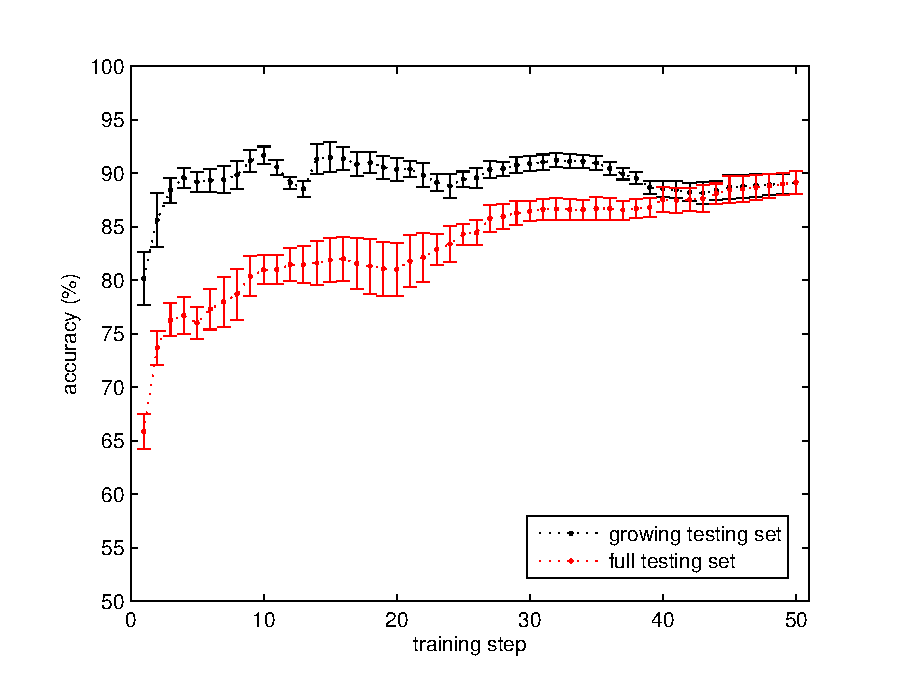
\includegraphics[width=0.45\textwidth]{figs/fig_resInc_OU21} &
    \includegraphics[width=0.45\textwidth]{figs/fig_growth_OU21} \\
    $(a)$ & $(b)$ \\
  \end{tabular}
  \caption{$(a)$: classification accuracy of an SVM, as the training set
    grows according to the OU procedure. \emph{Black curve:}
    growing testing set; \emph{Red curve:} full testing set. $(b)$:
    size of the online uniformised training set: number of samples
    (upper plot), fraction of the whole training set (lower plot).}
  \label{fig:inc}
\end{figure*}

Consider first the black curve in pane $(a)$ of the Figure: it is
apparent that, already after $4$ training steps, that is after some
$6$ minutes, the system can classify with an accuracy of about $90\%$,
as it was the case in the preliminary analysis (accuracy $89.57 \pm
0.94$). Notwithstanding some oscillations, the accuracy remains
substantially constant over the whole test and, at the end, is still
$89.14. \pm 1.05$. Consider now the red curve, representing the
accuracy obtained by the same models but on the \emph{whole} testing
set: now the system is being tested on samples drawn from zones of the
input space it has not yet seen; and, as one would expect, the
accuracy steadily increases, and it finally catches up with that
obtained by testing on the growing testing set.

Consider now pane $(b)$ of the Figure: the upper plot shows the size
of the online uniformised training set as the sample acquisition
proceeds; the lower plot shows the same curve as a fraction of the
full training set size. As time goes on, the OU procedure is letting
the uniform training set grow less and less; the fraction of the full
training set (lower plot) becomes smaller and smaller, being around
$1.5\%$ at the end.

From this we conclude that $(a)$ OU is keeping the training set
remarkably small in absolute terms, and smaller and smaller
percentage-wise, as more and more data is acquired; $(b)$ OU is
``letting in'' only relevant information, since the accuracy is
uniformly high if tested on a growing testing set, and ever growing if
tested upon a full testing set.

In other words, the OU procedure is effective in building a compact and
accurate training set for SVM classification.

What about the other approaches and problems? Figure \ref{fig:allres}
shows an all-inclusive set of results for all problems and approaches
considered, and for various values of the minimum distance threshold,
$d$, which was fixed at $0.21$ in the previous experiment.

\begin{figure*}[!ht] \centering
  \begin{tabular}{cc}
    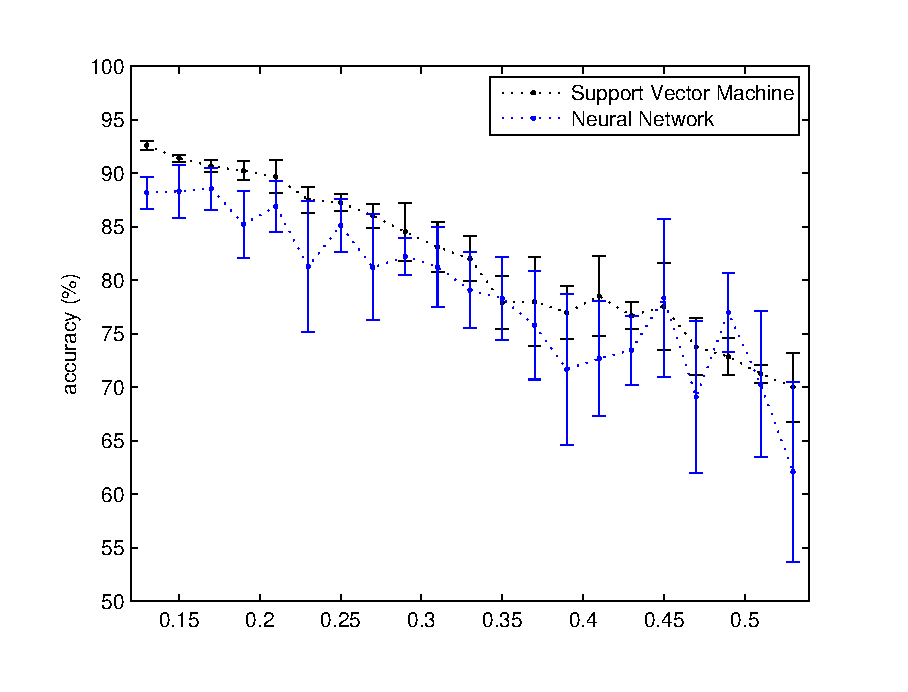
\includegraphics[width=0.45\textwidth]{figs/fig_all1} &
    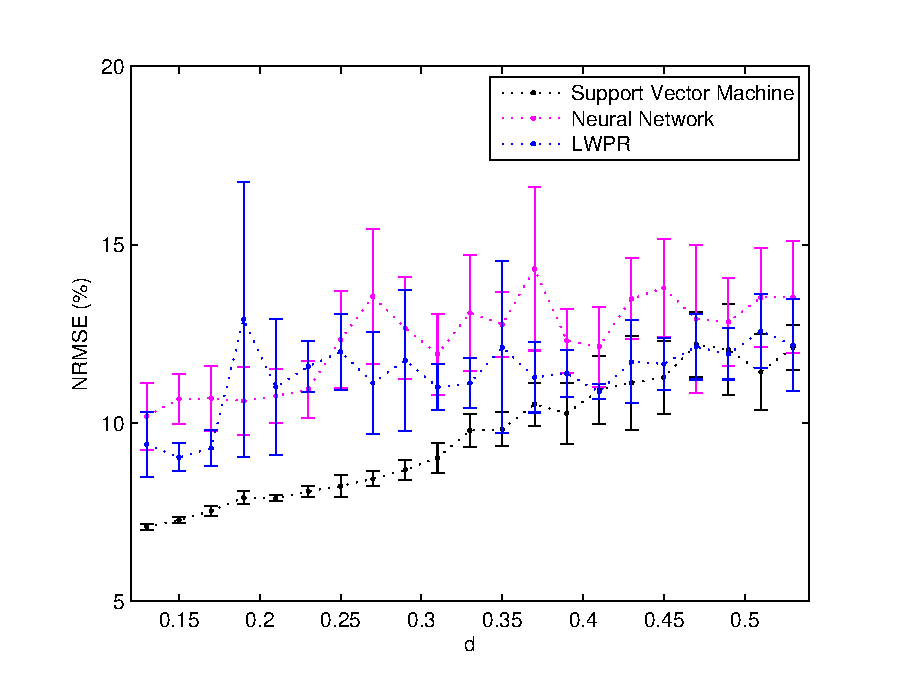
\includegraphics[width=0.45\textwidth]{figs/fig_all2} \\
    $(a)$ & $(b)$ \\
  \end{tabular}
  \caption{Classification and regression results using the OU
  procedure. $(a)$: classification, $(b)$: regression. Compare with
  Figure \ref{fig:TSsize} for the training set sizes.}
  \label{fig:allres}
\end{figure*}

As $d$ is increased from $0.13$ to $0.53$, all approaches show a
decreasing performance, as expected: in classification, the SVM is
almost uniformly better, going from $92.61\%$ for $d=0.13$ to
$70.01\%$ for $d=0.53$. The standard deviations for the SVM are, also,
uniformly smaller. In regression, again, the SVM is uniformly better
than the other approaches, ranging from $7.09\%$ NRMSE to $12.12\%$,
and it also shows uniformly smaller standard deviations. In both
problems, however, it must be remarked that the error bars largely
overlap, at least for $d>0.3$ in classification and $d>0.4$ for
regression.

One last consideration: as $d$ is increased, the size of the training
sets decreases like $d^{-10}$, since we are building a finite
partitioning of a subset of $\RR^{10}$ (see also Figure
\ref{fig:TSsize}, in which the training set size is plotted as a
function of $d$); whereas, it seems that the accuracy of all
approaches, and in both problems, only decreases linearly. This is a
remarkable feature of the OU procedure, since it will always be
possible to choose a polynomially smaller training set, for which we
can train a machine which will be only linearly worse.

\begin{figure}[!ht] \centering
  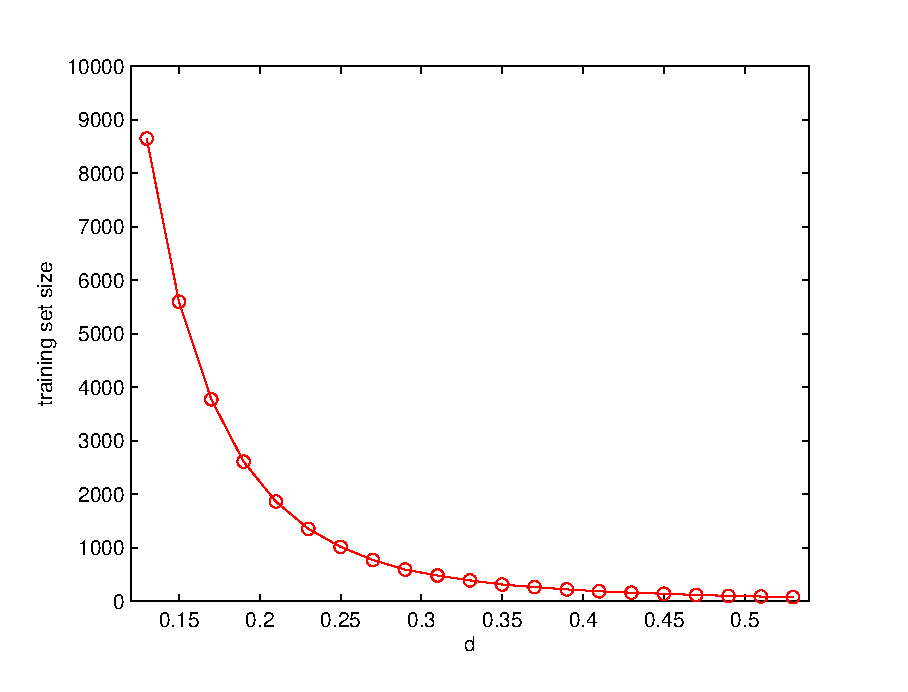
\includegraphics[width=0.45\textwidth]{figs/fig_allSize} \\
  \caption{Online uniformised training set size as $d$ changes.}
  \label{fig:TSsize}
\end{figure}

As a matter of fact, consider once again Figure \ref{fig:allres}, pane
$(b)$: at the far right end we have a SVM which has a still acceptable
error of $12.12\% \pm 0.64\%$, but whose training set, averaged over
the $5$ splits, consists of $77.4$ samples out of the original
$153000$!


\subsection{Application to a robotic 4-finger hand}
\label{subsec:application}
The method described above has been used for the control of the DLR
four-finger hand II \cite{ButFisGre2004}. This is a four-finger hand
with thirteen active degrees of freedom: three per finger, and one for
opposition of the thumb.  In the four identical fingers, the motion of
the third phalanx is coupled to that of the second. The actuation
system consists of brushless DC motors, tooth belts, harmonic drive
gears and differential bevel gears in the base joint. The differential
joint allows the use of full power of the two actuators for flexion or
extension, thus allowing the use of optimally small motors, obtaining
30N force at the finger tip. The high joint speed of over
360$^\circ$/s allows for high finger speed, important for, e.g., ball
catching. Besides force and position sensors, we use joint torque
sensors and specially designed potentiometers in each joint.
Furthermore, a tiny six-dimensional force/torque sensor is used in the
finger tip.

\begin{figure}
  \includegraphics[width=\columnwidth]{figs/egg-in-hand.jpg}
  \caption{The robotic four-finger hand controlled with EMG interface, exerting the right force to hold an egg.}
  \label{fig:egg-hand}
\end{figure}

In the EMG experiment, we used impedance control to exert a force as
generated by the EMG system to hold and grasp object. Example use of
the interface is demonstrated in figure~\ref{fig:egg-hand}. During the
experiment, we verified that the correlation coefficient between the
force applied by the subject and the robot was never less than $80\%$
over a time window of 10 seconds, which let us say that the force
applied by the robot was almost proportional to that applied by the
human subject.


\section{Discussion and Conclusions}
\label{sec:discussion}
Our experimental results, performed on a large data set of about
$153,000$ samples, clearly show that Online Uniformisation can be used
to obtain dramatically smaller training sets with no
\emph{qualitative} loss of information; in other words, as more of the
input space is sampled, OU keeps the training set up-to-date and
small. OU sets will result in small (and therefore, fast) and accurate
models of the sought-for EMG-to-hand map. Remarkably, OU works fine
for both grasp classification and force regression, and with all three
different machine learning approaches tested. Moreover, it is
extremely simple, being nothing more than an online check of Euclidean
distance in the input space. This check is done so far by considering
the new sample's distance from all samples in the current training
set, and therefore could become unfeasibly heavy as the set grows; but
the same check can be clearly done in constant time using an
algorithmic optimisation, such a hash table.

Moreover, OU will produce models which perform \emph{uniformly} well,
enabling a patient to drive the prosthesis with a good accuracy in
\emph{all} situations that might arise, no matter how frequently they
appear during the training phase.

The choice of the minimum inter-sample distance $d$ is obviously
crucial and depends on the required accuracy in classification and/or
regression; but as we have seen, as $d$ is increased, the machine's
performance degrades only linearly, whereas the training sets become
polynomially smaller. Therefore, at the price of having a slightly
worse performance, dramatically smaller training sets can be used.

To sum up, in this paper we have presented a machine learning
approach to joint classification of grasping and regression on the
applied force, using forearm surface electromyography. The approach is
totally non-invasive, easy to set up and use and it can be applied
from scratch with no previous knowledge of the problem. The Online
Uniformisation procedure can be used to incrementally build a training
set which will result in small and accurate models of the problem.

Our experiments, carried out using a Support Vector Machine with
Gaussian kernel, a Neural Network with sigmoidal activation function
and Locally Weighted Projection Regression, indicate that the approach
achieves, using a training set of about $1800$ samples on a total of
$153,000$ (for $d=0.21$), an average accuracy of around $90\%$ in
classification of grasp types and a normalised root MSE of $7.89\%$ in
prediction of the force applied during the grasp. Of the tested
approaches, SVM is marginally better than the others, especially when
larger training sets are used. The OU procedure is able to find as
small a training set as $77.4$ samples on average (out of $153,000$),
which will still result in a SVM having a remarkable NRMSE of
$12.12\%$.

\subsection*{Future work}

We believe this is the first step toward the real application of
machine learning to an EMG-driven adaptive, dexterous AHP. Let us
consider the problems outlined in section
\ref{subsubsec:electrodes}: in this paper we have solved problems
$3$ and $4$. Now, since OU lets us obtain good accuracy with extremely
small training sets, it is not too far-fetched to say that the
solution of problem $2$ is at hand --- in principle, the changing arm
posture can be taken into account simply by sampling more of the input
space. As far as problem $1$ is concerned, inter-subject usability is
really of lesser interest, since one patient only is supposed to ever
wear a prosthesis; on the other hand, multi-subject analysis has to be
carried out eventually, since it must be possible to obtain good
results on \emph{any} subject the method is applied to. We see no
reason, however, why this should not be the case, at least as far as
able-bodied subjects are concerned.

The ultimate problem is of coruse that of training the system upon
amputees. First of all, the patient must still have a good deal of
muscular and nervous plasticity in her arm stump; then, a smart way of
collecting training data must be devised --- an amputee is obviously
not expected to train the machine with a hand. A simple idea is that
of gathering EMG data from the patient's stump and grasping/force data
from her healthy hand, while instructing her to imagine doing the same
actions with both hands. Secondly, the issue of sensorial feedback
will have to be addressed, in order to provide the patient with
reliable information about the force actually involved in the
grasp. This is likely to be crucial in order to realise a tighter and
tighter loop between the patient and the prosthesis.

As far as force regression is concerned, the results presented above
are, to the best of our knowledge, totally novel. Surprisingly,
regression from the forearm surface EMG signal to the force applied by
the hand had never been attempted before. Given the good performance
obtained by our models, we claim that the relationship between the EMG
signal and the force has been captured by the models, under variable
conditions of muscle fatigue (within one session) and electrode
displacement (within sessions belonging to different groups). In a
certain sense, this work is an evolution of the so-called
\emph{proportional} control of myoelectric prostheses already
available on the market; in proportional control, the ``claw'' of the
prosthesis is actuated with a force which is proportional to the
amplitude of the EMG signal. In this case, the applied force is
proportional as well, but the control is realised in a totally natural
way, and is \emph{adaptive} to the user, what has never been done
before.


\section*{Acknowledgments}

This work is partially supported by the project NEURObotics,
FP6-IST-001917.

{\small
\bibliographystyle{IEEEtran}
%\bibliographystyle{spbasic}
\bibliography{paper}
}

%% \begin{IEEEbiography}{\includegraphics[width=1in,height=1.25in,clip,keepaspectratio]{claudio}}{Claudio Castellini}
%% biography
%% \end{IEEEbiography}

%% \begin{IEEEbiography}{\includegraphics[width=1in,height=1.25in,clip,keepaspectratio]{patrick}}{Patrick van der Smagt}
%% biography
%% \end{IEEEbiography}

\end{document}
